\documentclass[border=4pt]{standalone}
% Shared typography and colours for the standalone figures.
\usepackage{unicode-math}
\setmainfont{TeX Gyre Termes}
\setmathfont{TeX Gyre Termes Math}
\usepackage{tikz}
\usetikzlibrary{arrows.meta,positioning,calc,decorations.pathreplacing}
\usepackage{pgfplots}
\pgfplotsset{compat=1.18}

% One colour per element or subsystem. Record the mapping in
% the working repository conventions and use it identically in every figure.
\definecolor{elemA}{HTML}{1F5FA8}
\definecolor{elemB}{HTML}{B8461B}
\definecolor{elemC}{HTML}{2E7D32}
\definecolor{elemD}{HTML}{6A4C93}
\definecolor{frameline}{HTML}{555555}


\begin{document}
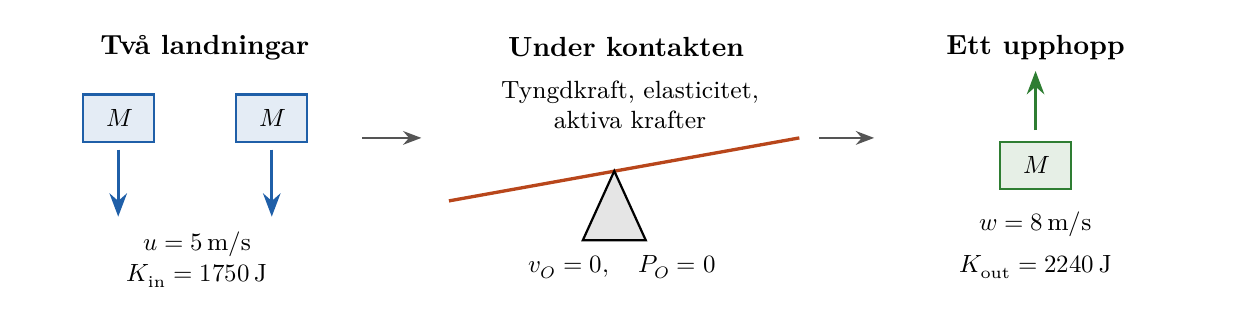
\begin{tikzpicture}[>=Stealth,font=\small]
\path[use as bounding box] (0,-.2) rectangle (15,3.1);
\node[font=\bfseries] at (2.25,2.85) {Två landningar};
\node[font=\bfseries] at (7.6,2.85) {Under kontakten};
\node[font=\bfseries] at (12.8,2.85) {Ett upphopp};
\foreach \x in {1.15,3.1}{
 \draw[fill=elemA!12,draw=elemA,thick] (\x-.45,1.65) rectangle (\x+.45,2.25);
 \node at (\x,1.95) {$M$};
 \draw[->,elemA,very thick] (\x,1.55)--(\x,.7);
}
\node at (2.15,.35) {$u=5\,\mathrm{m/s}$};
\node at (2.15,-.05) {$K_{\rm in}=1750\,\mathrm J$};
\draw[very thick,elemB] (5.35,.9)--(9.8,1.7);
\draw[fill=frameline!15,thick] (7.45,1.28)--(7.05,.4)--(7.85,.4)--cycle;
\node[align=center] at (7.65,2.12) {Tyngdkraft, elasticitet,\\aktiva krafter};
\node at (7.55,.06) {$v_O=0,\quad P_O=0$};
\draw[->,frameline,thick] (4.25,1.7)--(5,1.7);
\draw[->,frameline,thick] (10.05,1.7)--(10.75,1.7);
\draw[fill=elemC!12,draw=elemC,thick] (12.35,1.05) rectangle (13.25,1.65);
\node at (12.8,1.35) {$M$};
\draw[->,elemC,very thick] (12.8,1.8)--(12.8,2.55);
\node at (12.8,.6) {$w=8\,\mathrm{m/s}$};
\node at (12.8,.06) {$K_{\rm out}=2240\,\mathrm J$};
\end{tikzpicture}
\end{document}
